% Experiments Section
% User study data - single source of truth (DRY!)
% Study parameters
\newcommand{\NumParticipants}{41}

% Win rates
\newcommand{\OursQOne}{70}
\newcommand{\ATIQOne}{24}
\newcommand{\ReVideoQOne}{1}
\newcommand{\GWTFQOne}{5}

\newcommand{\OursQTwo}{71}
\newcommand{\ATIQTwo}{24}
\newcommand{\ReVideoQTwo}{2}
\newcommand{\GWTFQTwo}{3}

\newcommand{\OursQThree}{69}
\newcommand{\ATIQThree}{25}
\newcommand{\ReVideoQThree}{1}
\newcommand{\GWTFQThree}{5}

% Helper to convert percentage to decimal for plots
\newcommand{\pct}[1]{\fpeval{#1/100}}


\section{Results}
\label{sec:experiments}

\subsection{Implementation Details}

We use CogVideoX-5B~\cite{cogvideox2024} as our base text-to-video model for both the finetuned counterfactual video generation model and the V2V editing model.
Training was conducted on 8 H100 GPUs for one week using standard latent diffusion training with L2 loss.
We set $\Fframes = 49$,
with input resolution of $480 \times 720$ pixels,
corresponding to latent dimensions of $60 \times 90$.
We use $\Nblobs$ varying between 1 and 64 during training and set the control branch depth appropriately.
We use a learning rate of $10^{-4}$ and a dataset size of $100,000$ videos,
for $15,000$ iterations with an effective batch size of $32$.
We use an internal video dataset with 500,000 samples.
%\todo{fill number of samples}


\begin{comment}

USER STUDY
We conducted a user study to evaluate out algorithm.
We compared against ATI [cite], which is based on a newer base model WAN2.1 14B and operates on first-frame+motion-control-to-video
We manually created 20 videos
We had 10 participants
We asked them Q1: "Which video better preserves the input video's content?"
and Q2: "Which video better reflects the desired motion?"
and Q3: "Which video is overall a better edit of the input video?"

The results are in table TABLE1

TABLE1
	User Study
	[Ours] [ATI]
Q1: 70%    30%
Q2: 70%    30%
Q3: 70%    30%
[Caption: Users prefred ours yadda yadda]


QUANTITIVE EVALUATION:

We also created a qunantitative evaluation where we use photometric losses to gauge how good ours is against ATI
We created a dataset of 100 videos. We need to get counterfactual / ground truth pairs, so for each video we create an input and ground truth video as follows:
[potentially choose different variable names if it makes it more coherent] Given a test video v, we split v in the middle temporally to get v0 and v1. We then reverse v1 to get v1', so now the end of v0 is the start of v1'. We use v0 as the input video, and then choose 25 random points in that video the same way we do during training [ you can give tiny detail with better notation here]
For these 100 videos, we chose videos that have content exposed in the middle of the video that is not visible in the first frame, by choosing videos where there is a significant number of points that when tracked from the middle frame bidirectionally go missing in the first and last frames. [maybe we'll give again, a tiny equation here with notation - but only if you're confident you're doing it right]
For each algorithm we compare algo(v0) vs v1 using L2 loss on every frame.

TABLE1
	Photometric Loss
	[Ours] [ATI]
L2: .2    .5
[caption: ours had better photometric losses yadda yadda]

\end{comment}

% Additional macros for experiments
\newcommand{\Vtest}{V_{\text{test}}}     % test video
\newcommand{\Vzero}{V_0}                 % first half of test video  
\newcommand{\Vone}{V_1}                  % second half of test video
\newcommand{\Voneprime}{V_1'}            % reversed second half
% \newcommand{\Lphotometric}{\mathcal{L}_{\text{photo}}} % photometric loss (removed)
\newcommand{\Ntest}{N_{\text{test}}}     % number of test videos
\newcommand{\Npoints}{N_{\text{points}}} % number of tracking points for evaluation


We evaluate our motion editing approach through user studies and quantitative metrics, comparing against state-of-the-art motion control methods. %Details of how these baselines are implemented can be found in the appendix.

%\TODO{Explain how each baseline algorithm (ATI, ReVideo, Go-with-the-Flow, MotionPrompting) was implemented to work with our evaluation framework and track inputs. ---- PUT THAT IN APPENDIX }

\subsection{User Study}

We conducted a user study comparing our method against three baselines: ATI~\cite{ati},
a trajectory-guided image-to-video method based on WAN 2.1~\cite{wan};
ReVideo~\cite{revideo2024};
and Go-with-the-Flow (GWTF)~\cite{gowiththeflow2025}.
We manually created 20 test videos spanning diverse scenarios including object motion editing,
camera motion changes,
and complex scenes with multiple moving elements. \NumParticipants{} participants compared all four methods using the interface shown in the Supplementals,
selecting the best video for each of three questions per test case:
\begin{itemize}
    \item \textbf{Q1:} ``Which video better preserves the input video's content?''
    \item \textbf{Q2:} ``Which video better reflects the desired motion?''
    \item \textbf{Q3:} ``Which video is overall a better edit of the input video?''
\end{itemize}


\begin{table}[h]
\centering
\small
\begin{tabular}{l|cccc}
\hline
Question & Ours & ATI & ReVideo & GWTF \\
\hline
Q1: Content ($\uparrow$) & \textbf{\OursQOne\%} & \ATIQOne\% & \ReVideoQOne\% & \GWTFQOne\% \\
Q2: Motion ($\uparrow$) & \textbf{\OursQTwo\%} & \ATIQTwo\% & \ReVideoQTwo\% & \GWTFQTwo\% \\
Q3: Overall ($\uparrow$) & \textbf{\OursQThree\%} & \ATIQThree\% & \ReVideoQThree\% & \GWTFQThree\% \\
\hline
\end{tabular}
\caption{\textbf{User study win rates across all methods.}
Participants selected the best video for each question.
Our method consistently wins across all evaluation criteria.}
\label{tab:user_study}
\end{table}

Table~\ref{tab:user_study} show that users consistently ranked our method highest across all questions,
with win rates around 70\% compared to 25\% for ATI and less than 5\% for ReVideo and GWTF,
demonstrating superior content preservation and motion control.

\subsection{Quantitative Evaluation}

We developed a quantitative evaluation protocol using photometric reconstruction error to assess motion editing quality. 

\subsubsection{Dataset Construction}

We curated a dataset of $\Ntest = 100$ test videos using the following protocol.
Given a source video $\Vtest$ of length $\Ffull$ frames,
we split it temporally at the midpoint to obtain $\Vzero = \Vtest\left[1:\Ffull/2\right]$ and $\Vone = \Vtest\left[\Ffull/2:\Ffull\right]$.
We then create the counterfactual input by temporally reversing $\Vone$ to get $\Voneprime$,
ensuring temporal continuity between $\Vzero$ and $\Voneprime$ (i.e., the last frame of $\Vzero$ matches the first frame of $\Voneprime$).

We selected random internet videos not seen during training where significant content appears in middle frames but is not visible in the first frame.
To quantify this,
we initialize $\Npoints = 25$ tracking points at the temporal midpoint of each video and track them bidirectionally using TAPNext~\cite{tapnext}.
We retain only videos where a substantial number of points become occluded when tracked to both the first and last frames.

\begin{figure}[htb]
    \centering
    \includegraphics[width=\linewidth]{successive_edit_horz.pdf}
    \caption{\textbf{Iterative editing.}
Outputs can become inputs for subsequent edits,
enabling complex sequential motion changes. Yellow dots used for first edit, green/cyan for second. Arrows added from old to new position for ease of visualization. }
    \label{fig:iterative_editing}
\end{figure}


\subsubsection{Evaluation Protocol}

For each test case,
we use $\Vzero$ as input and $\Vone$ as the target video.
We provide both our method and ATI with identical motion trajectories extracted from $\Vone$ and measure reconstruction quality using frame-wise L2 loss:

\begin{equation}
L_2 = \frac{1}{\Fframes} \sum_{i=1}^{\Fframes} \|I_i^{\text{pred}} - I_i^{\text{target}}\|_2^2
\end{equation}

where $\Fframes$ is the number of frames,
$I_i^{\text{pred}}$ is the $i$-th predicted frame,
and $I_i^{\text{target}}$ is the corresponding target frame.

\begin{table}[h]
\centering
\begin{tabular}{l|c|c|c}
\hline
\textbf{Method} & $\mathbf{L_2}\,(\downarrow)$ & \textbf{SSIM}\,($\uparrow$) & \textbf{LPIPS}\,($\downarrow$) \\
\hline
Ours               & \textbf{0.024} & \textbf{0.098} & \textbf{0.031} \\
ATI                & 0.038 & 0.094 & 0.072 \\
Go-with-the-Flow   & 0.067 & 0.089 & 0.088 \\
ReVideo            & 0.096 & 0.080 & 0.106 \\
\hline
\end{tabular}

\caption{Evaluation of photometric reconstruction error for our method and ATR. Our method achieves significantly lower L2 reconstruction error.}
\label{tab:quantitative}
\vspace{-10pt}
\end{table}

Our method achieves substantially lower reconstruction error (Table~\ref{tab:quantitative}),
confirming that our full-video approach better preserves content compared to first-frame generation methods,
particularly in scenarios involving content not visible in initial frames.

\subsection{Qualitative Comparisons}

\noindent \textbf{Iterative Edits.}
One of the strengths of our technique is that it can be applied iteratively - taking the output of one run and using it as input for a successive video edit. This allows users to chain multiple simple, intuitive edits together in order to achieve a very complicated edit. This iterative editing also provides more immediate feedback to the user making the process more transparent and easier to control. In~\cref{fig:iterative_editing}, we show that a complex edit (an object motion and a camera change) can be decomposed into its core parts and applied one by one. While this example demonstrates some degree of subject drift, this can be attributed in part to the quality of the base video model. We believe that future versions of our method will be able to be applied infinitely.

\begin{figure*}[t]
    \centering
    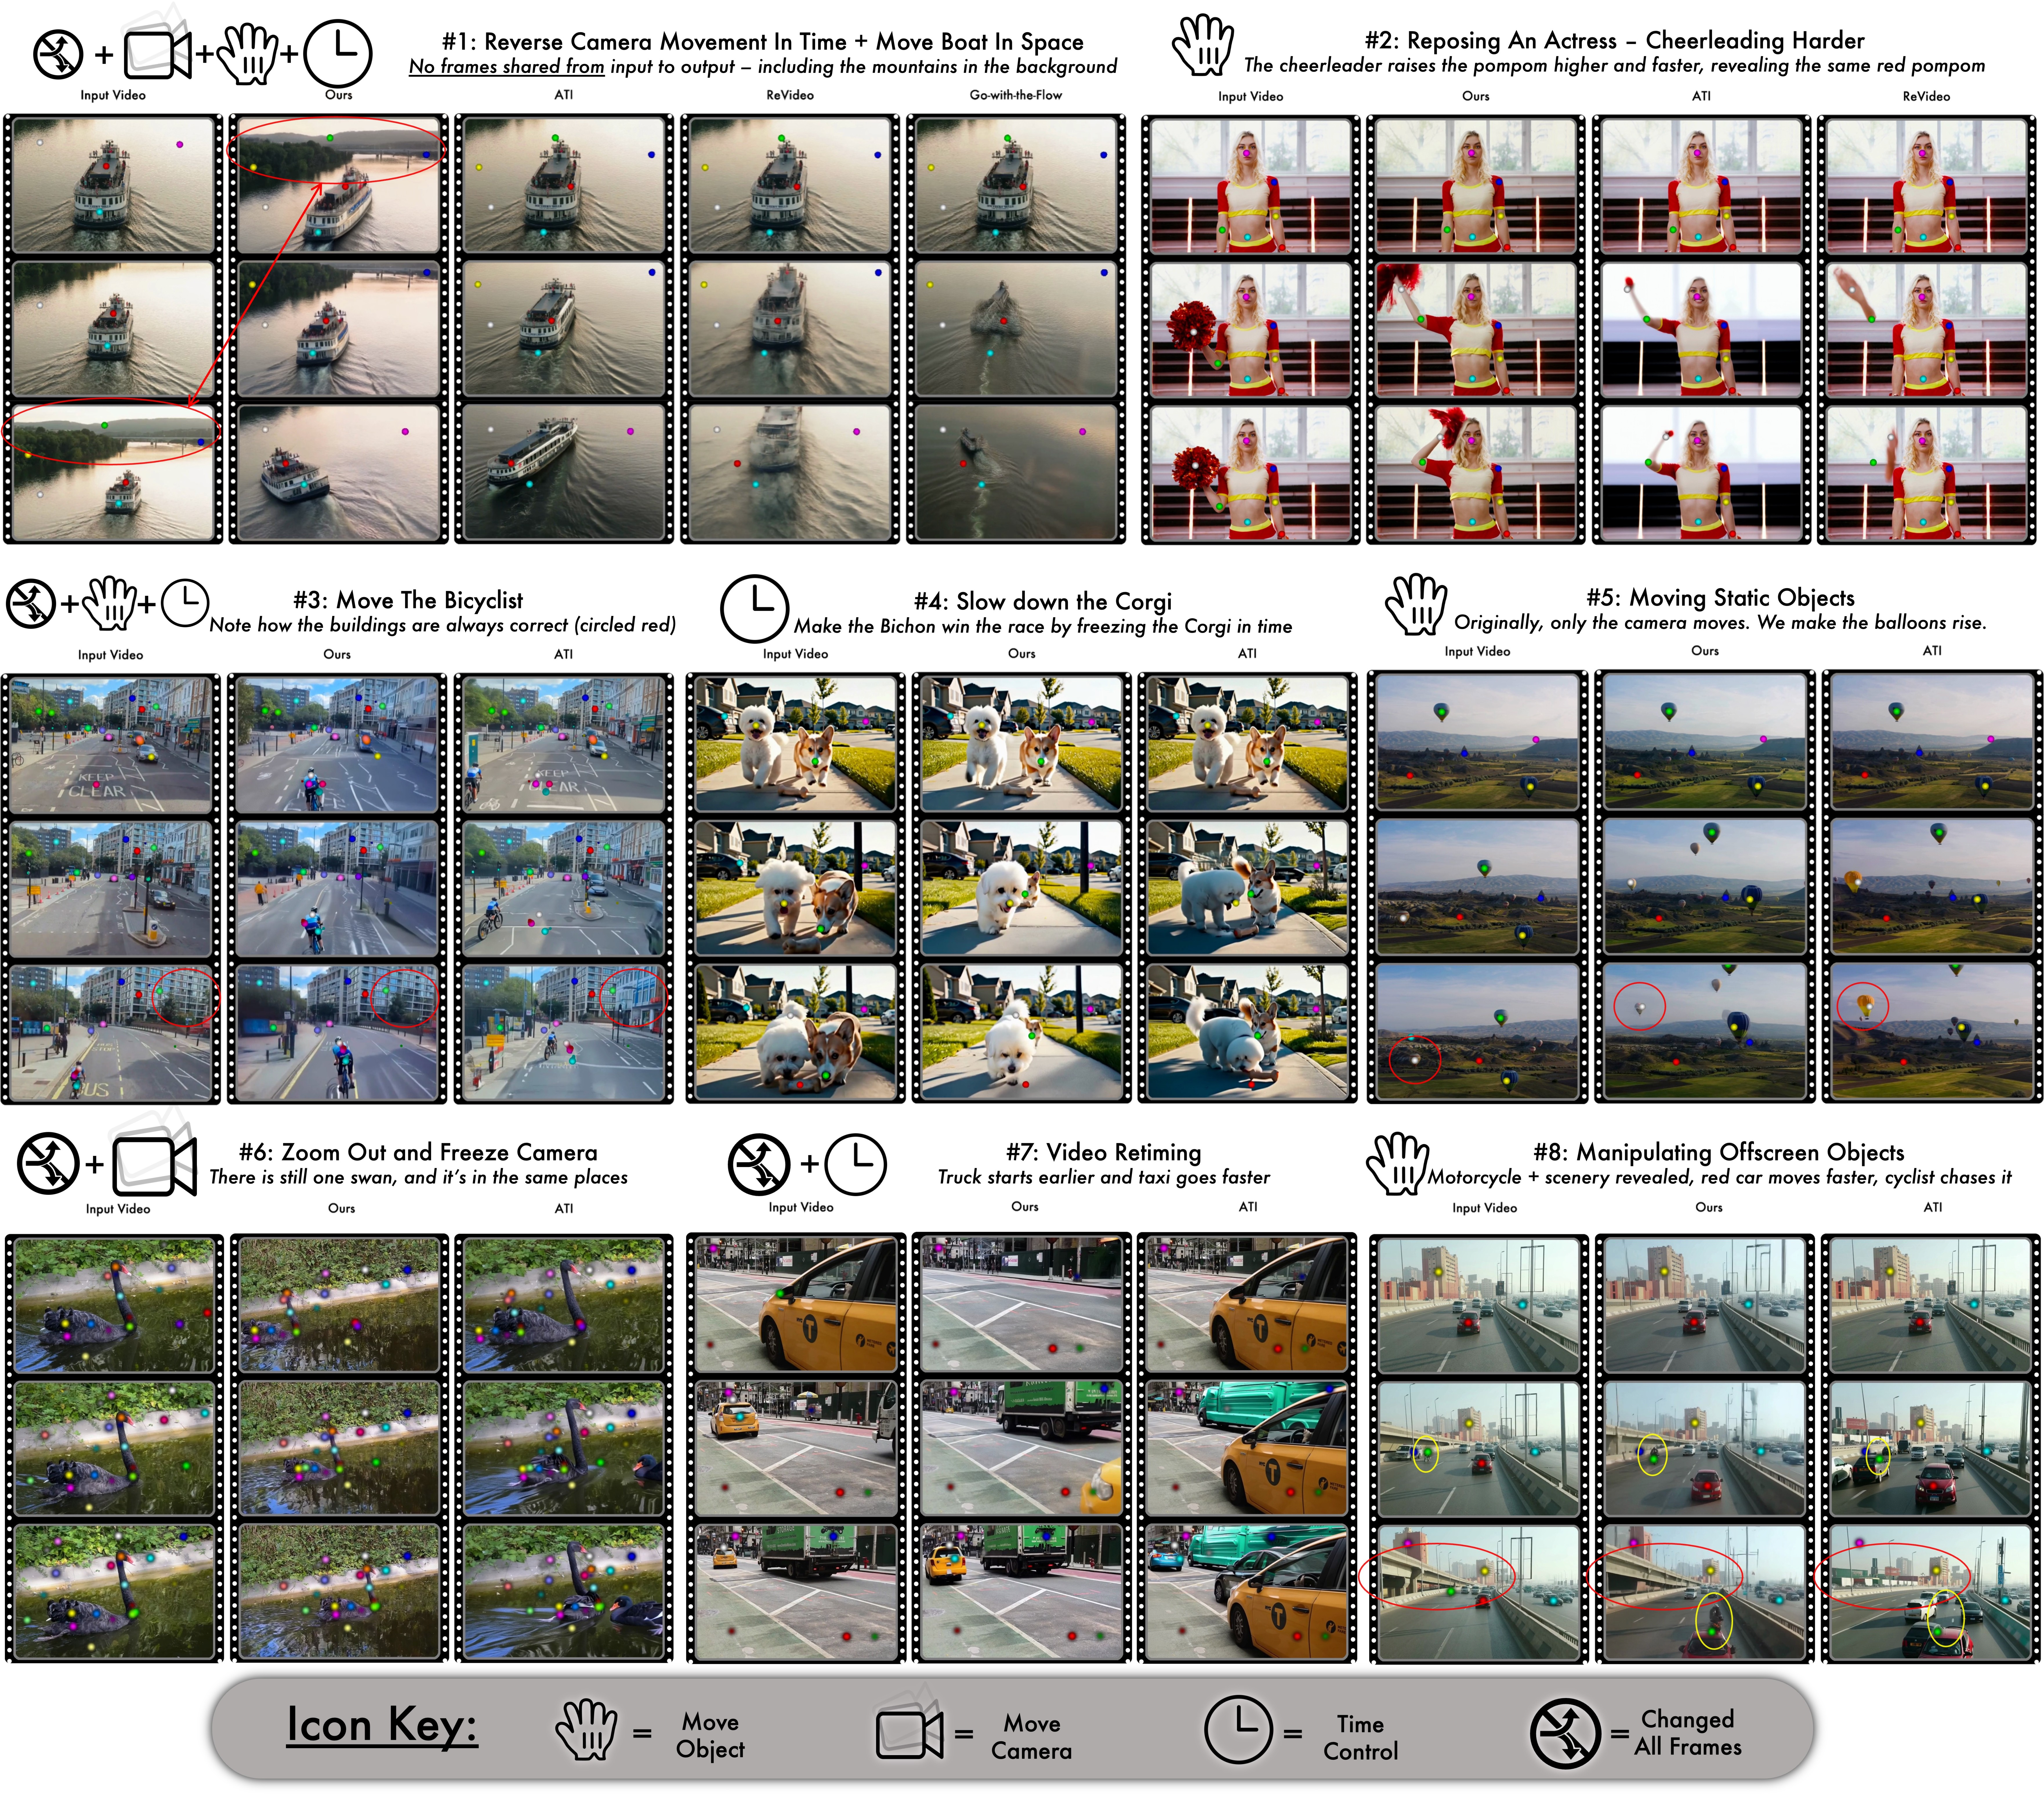
\includegraphics[width=1\linewidth]{megacomparisonfigurev2.jpg}
    % \includegraphics[width=1\linewidth]{\figfolder/MegaComparisonFigurev2}
    \caption{Comparison of our method vs.\ baselines across eight challenging motion editing scenarios.
Each row shows a different editing task with input video,
our result,
and ATI's result (with additional baselines shown for subfigure 4).
\textbf{Icon key:} Human Pose (modifying human motion),
Move Object (repositioning objects),
Move Camera (changing camera motion),
Time Control (retiming events),
Changed All Frames (no shared frames between input/output—impossible for image-to-video methods).
Colored dots track correspondence points throughout the video;
dot presence/absence indicates object visibility.
Red circles highlight key differences where baselines fail.}
    \label{fig:mega_comparison}
\end{figure*}

\noindent\textbf{Baseline comparisons.} Figure~\ref{fig:mega_comparison} compares our method against several baselines in multiple video editing scenarios, each of which demonstrate the capabilities of our motion edits. We primarily compare against ATI~\cite{ati},
a trajectory-guided image-to-video method based on WAN 2.1~\cite{wan},
our strongest baseline despite using a more powerful base model than our CogVideoX base.
Subfigure 4 additionally shows ReVideo~\cite{revideo2024} and Go-with-the-Flow~\cite{gowiththeflow2025},
which rated poorly in user evaluation—ReVideo lacks text conditioning and Go-with-the-Flow was not designed for point control.


\noindent\textbf{Edit \#1: Complex Edits on the Boat Scene.} This edit moves the boat left and shifts the camera so that mountains from the original's last frame appear in the edit's first. This requires specifying a substantial temporal trajectory change and holistic knowledge of the scene content. Ours is the only method that realistically moves the boat while correctly adjusting the camera to reveal the mountains at the beginning of the video.

\noindent\textbf{Edit \#2: Reposing a Cheerleader.} This edit raises the cheerleader's arms. The challenge involves preserving the red pom-pom, which is absent from the first frame. Ours successfully modifies the motion while retaining this content. In contrast, ATI and ReVideo rely solely on the first frame, leading to unnatural movements and a failure to preserve the pom-pom.

\noindent\textbf{Edit \#3: Move The Bicyclist.} This edit controls a cyclist visible only in the final frame of the original video. Ours correctly propagates the cyclist and tracking dots (cyan, magenta, white) throughout. ATI, lacking full temporal context, misplaces the cyclist and synthesizes wrong buildings (red circles).

\noindent\textbf{Edit \#4: Dog Race.}
Differential timing breaks single-frame-based methods. We decelerate the Corgi (green dot) to reverse the race outcome while keeping the Bichon steady. This requires independent temporal control; ATI fails to decouple the motions, incorrectly copying the Bichon and transforming a light pole into a tree.

\noindent\textbf{Edit \#5: Moving Static Balloons.}
We add upward motion to stationary balloons. The white balloon (white dot), which appears mid-video, challenges partial information methods. While ATI moves visible balloons, it renders the initially hidden white balloon orange due to missing appearance data. Our method uses full video context to maintain correct colors.

\noindent\textbf{Edit \#6: Zooming out on the Swan} 
In this DAVIS~\cite{davis2016} example, we transform a panning shot into a static, zoomed-out view. The output field of view differs entirely from the input, yet the swan must remain anchored to specific vegetation. Lacking full spatial context, ATI synthesizes a second swan and produces inconsistent motion.

\noindent\textbf{Edit \#7: Retiming a taxi.}
We do a complex isolated retiming of taxi and truck movement. This requires complete temporal understanding; ATI's single-frame generation cannot achieve this reversal. Figure~\ref{fig:mega_comparison} compares our method against ATI (WAN 2.1-based), as well as ReVideo and Go-with-the-Flow (in Subfigure 4), both of which were rated poorly due to their design limitations.

\noindent \textbf{Edit \#8: Moving an Offscreen Car.}
As the camera follows a red car, a motorcyclist enters late. We reposition this initially invisible rider behind the car while maintaining consistent background architecture. Lacking future frames to reference the rider and buildings (red circles), ATI synthesizes incorrect content.


\noindent\textbf{Discussion.}
These scenarios highlight I2V limitations: conditioning only on the first frame prevents leveraging information from the full input. Our V2V formulation enables bidirectional flow, allowing outputs to pull content from \emph{any} input frame. This handles offscreen content, camera changes, and reordering—challenges where I2V methods like ReVideo~\cite{revideo2024}, Go-with-the-Flow~\cite{gowiththeflow2025}, and MotionPrompting~\cite{motionprompt2024} fail.

% Additional comparison figures have been integrated into Figure~\ref{fig:mega_comparison}

%\begin{figure}[h]
%    \centering
%    \fullcompfig[1]{4}{\figfolder/FullComp_BlackSwan}
%    \caption{The camera is frozen while the black swan swims.}
%    \label{fig:comp_blackswan}
%\end{figure}
%
%\begin{figure}[h]
%    \centering
%    \fullcompfig[2]{5}{\figfolder/FullComp_Boat}
%    \caption{Editing the boat's trajectory and motion.\cih{todo: give categories / labels}}
%    \label{fig:comp_boat}
%\end{figure}
%
%\begin{figure}[h]
%    \centering
%    \fullcompfig[1]{4}{\figfolder/FullComp_Cheerleader}
%    \caption{Changing the motion of the cheerleader's pompoms.}
%    \label{fig:comp_cheerleader}
%\end{figure}
%
%\begin{figure}[h]
%    \centering
%    \fullcompfig[2]{4}{\figfolder/FullComp_Judge}
%    \caption{The judge walks in from the right with camera zoom.}
%    \label{fig:comp_judge}
%\end{figure}

%\begin{figure}[h]
%    \centering
%    \fullcompfig[1]{4}{\figfolder/FullComp_Candle}
%    \caption{A hand grabs the candle while the camera is stopped.}
%    \label{fig:comp_candle}
%\end{figure}

%\begin{figure}[h]
%    \centering
%    \fullcompfig[2]{4}{\figfolder/FullComp_CityBiker}
%    \caption{Editing the motion of an urban cyclist.\cih{a bit hard to see}}
%    \label{fig:comp_biker}
%\end{figure}
%
%\begin{figure}[h]
%    \centering
%    \fullcompfig[1]{4}{\figfolder/FullComp_Balloons}
%    \caption{Hot air balloons rise while the camera motion is slowed.}
%    \label{fig:comp_balloons}
%\end{figure}
%
%\begin{figure}[h]
%    \centering
%    \fullcompfig[1]{4}{\figfolder/FullComp_Dogs}
%    \caption{The corgi stays behind while the bichon moves forward.}
%    \label{fig:comp_dogs}
%\end{figure}

% \begin{figure}[h]
%     \centering
%     \includegraphics[width=1\linewidth]{\figfolder/FullComp_Shakycam}
%     \caption{Editing the camera motion on shaky footage. \cih{this just looks like brown}}    \label{fig:comp_shakycam}
% \end{figure}

